\documentclass[dvipdfmx]{jsarticle}
\usepackage{graphicx}[dvipdfmx]
\usepackage{multirow}
\usepackage{array}
\usepackage{amsmath,amssymb}
\usepackage{url}
\usepackage{listings}
\usepackage{color}
\usepackage{verbatim}

\title{計算機設計論 レポート課題:MIPSプロセッサの回路設計}
\author{1295149 森岡悠人\\}
\date{\today}

\begin{document}
\maketitle

\section{モジュール仕様書}

\section{動作検証}
作成したverilogコードがMIPSの命令セットを実行できるかどうかの検証を行った.
教科書\cite{textbook}に掲載されているアセンブラプログラム(load\_store, arithmetic, array, if\_then\_else, while, function, recursion, hanoi)を\texttt{IMem.txt}に書き込んでおき,IMに読み込ませ,modelsimを用いて動作のシミュレーションを行った.
シミュレーション結果は,display命令を用いて,PC, Instruction, ALU\_resultレジスタの内容を表示することで確認した.
シミュレーションには,modelsim 20.1を使用した.
シミュレーションの様子を図\ref{fig:simulation}に示す.

\begin{figure}[h]
\centering
  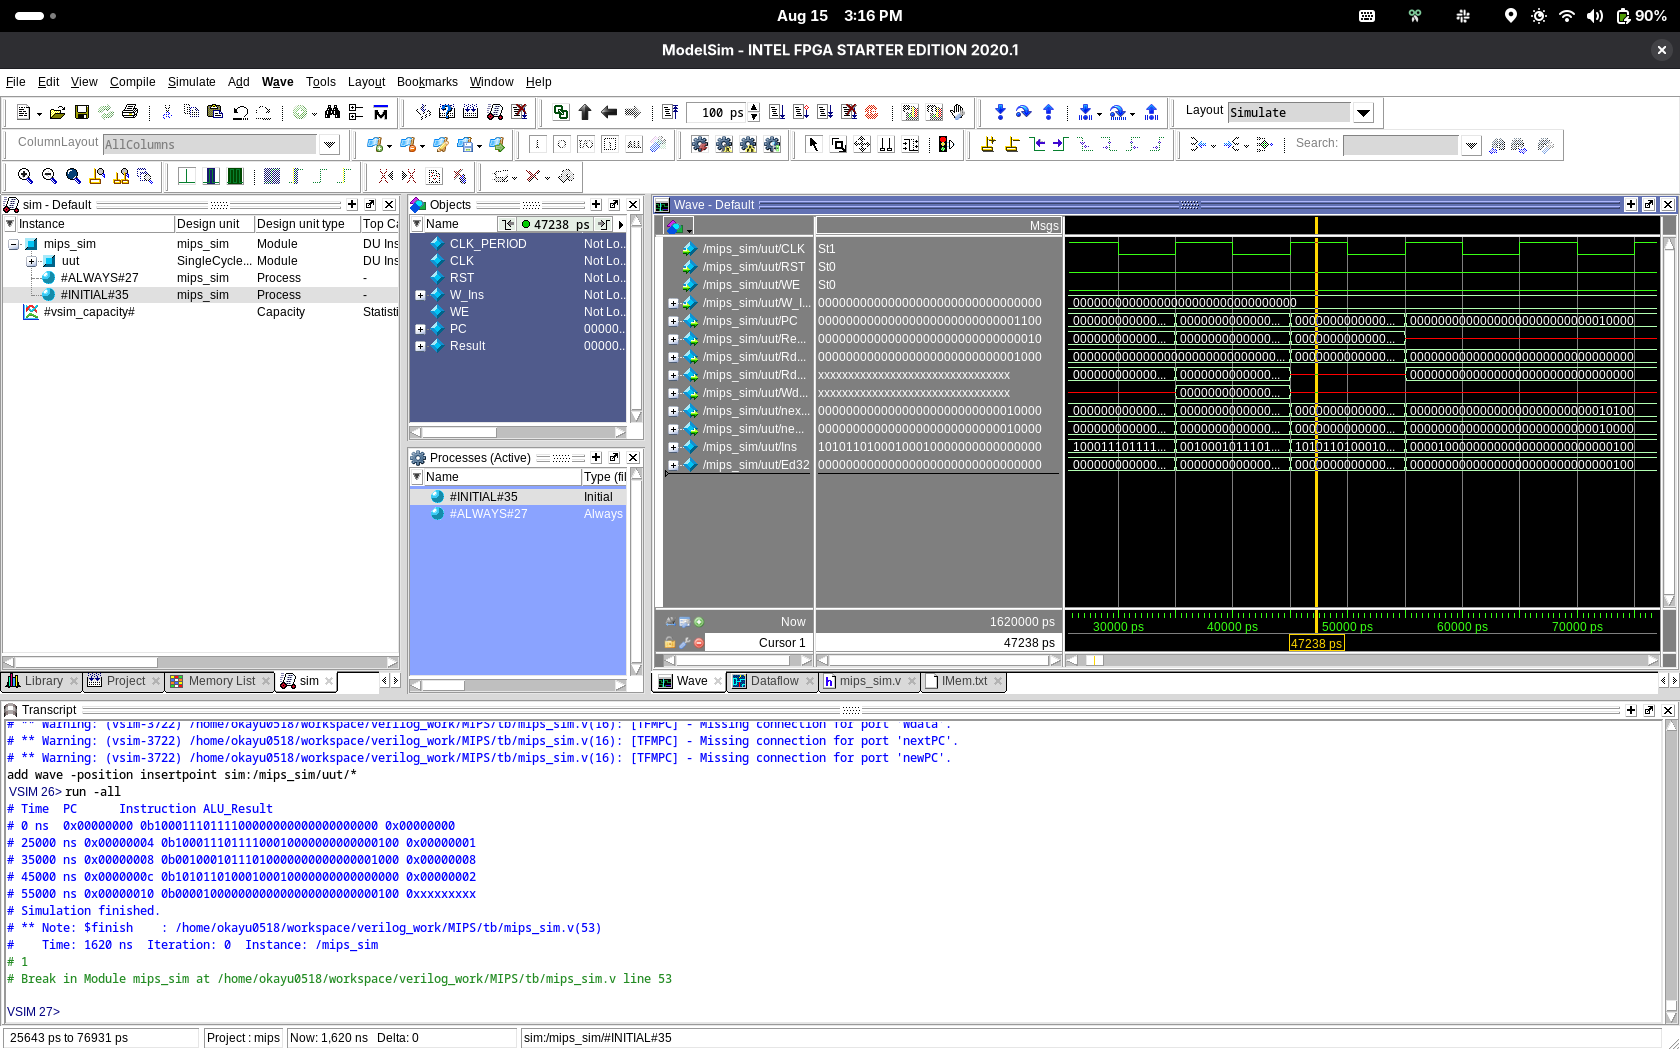
\includegraphics[width=0.8\textwidth]{modelsim.png}
  \caption{modelsimによるシミュレーションの様子}
  \label{fig:simulation}
\end{figure}

\subsection{test: load\_store}
\subsubsection{load\_storeのテスト結果}
\verbatiminput{test-results/load_store.txt}
\subsection{test: arithmetic}
\subsection{test: array}
\subsection{test: if\_then\_else}
\subsection{test: while}
\subsection{test: function}
\subsection{test: recursion}
\subsection{test: hanoi}


\section{考察}



\section{感想}



\bibliographystyle{junsrt}
\bibliography{refs}
\end{document}

